\documentclass[twocolumn,10pt]{article}

\usepackage[dvips]{graphicx}
%\usepackage{times}
\usepackage{fullpage}
\usepackage{eprint}
\usepackage{rotating}
\usepackage{eepic}
\usepackage{amsfonts}
\usepackage{algorithmic}
\usepackage{amsthm}

\theoremstyle{plain}
\newtheorem{theorem}{Theorem}

\title{Quantum Compiling with the Super-Kitaev Algorithm}
\date{February 11, 2011}
\author{Paul Pham}

\input{Qcircuit}

\begin{document}

%\newcommand{\ket}[1]{|#1 \rangle}
%\newcommand{\bra}[1]{\langle #1 |}
\newcommand{\braket}[2]{\langle #1|#2 \rangle}
\newcommand{\normtwo}{\frac{1}{\sqrt{2}}}
\newcommand{\norm}[1]{\parallel #1 \parallel}

\maketitle

\section{Abstract}

Quantum compilers will be needed to implement algorithms on an
80-qubit quantum computer being constructed in the next five years.
Like digital computers, quantum
computers need compilers to approximate high-level descriptions of
an algorithm using a low-level, universal, machine-dependent
instruction set. This work contributes
a numerical comparison of the
resources needed to run two separate quantum compiling algorithms, along
with the underlying open source code.
The first is the well-known Solovay-Kitaev theorem which showed that
efficient quantum compiling was possible in theory, but with some large
performance overheads in practice. The other is a
lesser-known result known as Super-Kitaev, which optimizes the compiled
circuit depth using parallelization at the expense of more ancilla qubits
and a larger overall circuit size. Finally, we discuss some implications for
future quantum architectures and also analog computers
(for when they come back into
fashion).


\section{Introduction}

Quantum computers can do some pretty amazing things in theory: they
can break the RSA cryptosystem using Shor's factoring algorithm,
ensure perfectly private communication,
do unstructured search, solve random walks, and
simulate quantum physical systems much more efficiently than classical
computers. But how
do we bridge the gap between algorithms that run on paper and those that
will soon run on actual machines being built in laboratories as we speak?
One important step in that direction is \emph{quantum compiling}, the
approximation of a high-level quantum algorithm description to a sequence
of low-level, universal quantum gates that depend on our hardware, the
"assembly language" of quantum computing.

When describing a quantum algorithm, we use a high-level formalism of
gates operating on qubits in the quantum circuit model.
We can treat gates operating on an $n$-qubit quantum computer as unitary
matrices of dimension $2^n \times 2^n$ with unit determinant.
However, in experimental settings,
we can only perform some gates efficiently, and these are local
two-qubit or single-qubit operations.
Moreover, most of our results for fault-tolerant
quantum computing in the presence of noise stipulates that we have a finite
number of universal gates we can perform with some limited precision.

Two quantum compiling algorithms are currently known. The first algorithm,
by Solovay and Kitaev \cite{Dawson2005},
is one of the central results of quantum computing which states that we
can approximate quantum gates efficiently without losing any performance
gains over classical computers.
The second result, which is more recent but much less well-known, improves
Solovay-Kitaev by making a time-space tradeoff and using parallelism
\cite{ksv02}.
Therefore, we call it Super-Kitaev (a name originated by Aram Harrow).

This work contributes the calculation of physical resources needed
to run these two quantum compiling algorithms, open source code to duplicate
these results available at \texttt{http://quantum-compiler.org},
and much needed publicity for Super-Kitaev.

The rest of this report is organized as follows.
First things first, Section \ref{sec:prelims} defines terms and parameters
so that we can discuss quantum compilers with some precision as well as
giving asymptotic bounds for specific algorithms.
Then Section
\ref{sec:related} gives a brief history of quantum compiling.
The next two sections describe the two compiling algorithms and how
to measure their relative performance.
Section \ref{sec:sk-algo} reviews the original Solovay-Kitaev result and
Section \ref{sec:main-algo} describes Super-Kitaev along with its
most resource-intensive modules. Section \ref{sec:methods} describe
our methods for the performance comparisons, which are given in Section
\ref{sec:results}. Finally, we make some comments about these results
and suggest future directions for extending this work. Ready? Let's go.

\section{Preliminaries}
\label{sec:prelims}

\subsection{Some Special Operator Notation}

Borrowing the notation in \cite{ksv02},
we can define two "meta-operators" which takes some unitary $U$ as
a parameter. The first describes a controlled-$U$ operation where the control
is some single qubit.

\begin{displaymath}
\Lambda(U) = \ket{0}\bra{0} \otimes I + \ket{1}\bra{1} \otimes U
\end{displaymath}

The second describes a registered-$U$ operation, which
can be thought of as controlled on some multi-qubit register $\ket{p}$
encoding an $m$-qubit number $p$ to apply $U$ a certain number of times to a
target
register.

\begin{displaymath}
\Upsilon_m(U) : \ket{p} \otimes \ket{\psi} \rightarrow \ket{p}
\otimes U^p\ket{\psi}
\end{displaymath}

\subsection{A Universal Set of Gates}

We use the following universal standard set of gates $\mathcal{G}$.
The single-qubit rotations about the $x-$ and $z-$ axes
(of which $X$ and $Z$
are special cases) are known to be efficient on ion trap
implementations, but the set of realizable angles $\theta$ is finite.

\begin{displaymath}
\mathcal{G} = \{ H, K, K^{-1}, X, Z,
\Lambda(\sigma_x), \Lambda^2(\sigma_x) \}
\end{displaymath}

$\Lambda(\sigma_x)$ and $\Lambda^2(\sigma_x)$ are CNOT and Toffoli,
respectively.
Any current or future physical implementations of a quantum
computer will need to efficiently implement this set or an equivalent one.
Without proving the universality of $\mathcal{G}$, we note that all known
quantum algorithms reduce to it.

\subsection{Parameters}

The problem of quantum compiling is to translate
an entire circuit $C$ of $L$ gates with depth
$d$ to a new, compiled circuit $C'$ of size $L'$ and depth $d'$ which approximates
$C$ within some error $\epsilon$ using some distance measure.

In our code, we use the trace measure introduced by Austin Fowler which disregards
the global phase factor, so that we don't waste time trying to approximate
the unmeasurable phase of our target gate. Here,
$l$ refers to the dimensionality
of our system (for $n = 2^l$ qubits).

\begin{equation}
d(U,\tilde{U}) = \sqrt{\frac{l - \norm{\mathrm{tr}(U^\dagger \tilde{U})}}{l}}
\end{equation}

We will be somewhat sloppy and use the terms ``error'', ``precision'', and
``accuracy'' interchangeably when approximating gates.
There is some overhead in the compiled circuit, so in
general $C'$ is larger (that is, $L' > L$ and $d' > d$). It's also known that
in order to approximate a circuit with $L$ gates to a total precision of
$\epsilon$
requires each gate to be approximated to a precision of
$n = O(\log(L/\epsilon)$. We'll call the classical preprocessing time to
produce $C'$ as $T$.
 
Circuit depth is a heuristic for how parallelizable our
circuit is. For example, in an ion trap, if we had multiple lasers,
we could ``flatten'' our circuit into layers with bounded fan-in and
fan-out and operate on multiple ions in parallel.
All other things being equal, a circuit with low depth will complete
faster than one with high depth, although in practice we can only execute
fixed-width circuits.

\subsection{Quantum Coprocessor Model}

All experimental implementations of quantum computers treat them as an
auxiliary device controlled by a classical computer. This is the way
quantum computers will function for the foreseeable future, and many
quantum algorithms can actually be split into classical and quantum parts
to reflect this distinction. For example,
Solovay-Kitaev is a completely classical algorithm which is run before
a quantum algorithm to yield a deterministic set of gates. Super-Kitaev
also contains classical postprocessing as part of its parallelized
phase-estimation. Since classical computers are well understood and
pretty fast, we will neglect the performance of these classical parts
if they are polynomial in time. However, we will discuss one aspect
of classical overhead later since it appears to be intractable.

\subsection{Asymptotic Bounds}

The Solovay-Kitaev and Super-Kitaev algorithms compile circuits with
a size and depth which depend on the desired precision via the
parameter $n$ as shown below. We'll see these asymptotic bounds reflected
later in the actual numerical results in Section \ref{sec:results}.
The version of Solovay-Kitaev in Section \ref{sec:sk-algo} has a
larger exponent for the logarithm but is
easier to understand.

\begin{center}
\begin{table}
\begin{tabular}{|c|c|c|}
\hline
   & Solovay-Kitaev & Super-Kitaev\\
\hline
$L'$ & $O(Ln^{3+\nu})$ & $O(Ln + n^2 \log n)$\\
$d'$ & $O(dn^{3+\nu})$ & $O(d \log{n} + (\log{n})^2))$\\ 
\hline
\end{tabular}
\end{table}
\end{center}

where $\nu$ is a small positive constant.
The improve Solovay-Kitaev with the improved $3+\nu$ exponent and
Super-Kitaev are both described in \cite{ksv02}.

%\section{Performance}

Just to get this out of the way, in case you are wondering whether to be
excited or not about Super-Kitaev.

\begin{tabular}{|c|c|c|}
\hline
   & Solovay-Kitaev & Super-Kitaev\\
$L'$ & $O(Ln^{3+\nu})$ & $O(Ln + n^2 \log n)$\\
$d'$ & $O(dn^{3+\nu})$ & $O(d \log{n} + (\log{n})^2))$\\ 
\hline
\end{tabular}

where $\nu$ is a small positive constant.
The remaining parameters are yet to be determined.



\section{Related Work}
\label{sec:related}

In 1995, Seth Lloyd found that almost any two distinct single-qubit rotations are
universal for approximating an arbitrary single-qubit rotation, but that this
approximation could be exponentially long in both time and length $T,L = (O(1/\epsilon))$ \cite{Lloyd1995}.

The theorem which is now called Solovay-Kitaev was discovered by Solovay in
1995 in an unpublished manuscript and independently later discovered by
Kitaev in 1997 \cite{nc00} which showed that $T,L = O(\log^c{1/\epsilon})$ for
$c$ between 3 and 4.

In 2001, Aram Harrow completed his undergrad thesis arguing that it would be difficult
to beat $c < 2$ for the above bounds using a successive approximation
method\cite{harrow01}.

In 2002, Kitaev, Shen, and Vyalyi published their book which contains an
application of parallelized phase estimation towards simulating a quantum
circuit (what we are calling Super-Kitaev) \cite{ksv02}.
That is, an alternative quantum compiler to Solovay-Kitaev which has
asymptotically better circuit depth and $T=O(1)$
but using ancillary qubits and increased
circuit size.

In 2003, Harrow, Recht, and Chuang demonstrated that a certain universal
set could be used to saturate the lower bound $L=O(\log{1/\epsilon})$
but it remains an open problem whether any efficient algorithm exists
which can do this in tractable $T$ \cite{hrc02}.

In 2005, Dawson and Nielsen published their pedagogical review
paper of Solovay-Kitaev \cite{Dawson2005}.

In 2010, Burrello, Mussardo, and Wan discovered a quantum compiler for
topological quantum computing which saturates the lower bound ($c=1$) for
non-Abelian anyons \cite{Burrello2010}.

\section{Review of Solovay-Kitaev}

Here I'll remind you of the basic pseudo-code for normal Solovay-Kitaev.
Our development is taken from the excellent review paper \cite{Dawson2005}.

\begin{algorithmic}[1]
\STATE \textsc{function} $\tilde{U}_n \leftarrow$ SOLOVAY-KITAEV$(U,n)$
\IF{$n == 0$}
\STATE $\tilde{U}_n \leftarrow $ BASIC-APPROX$(U)$
\ELSE
\STATE $\tilde{U}_{n-1} \leftarrow$ SOLOVAY-KITAEV$(U, n-1)$
\STATE $A,B \leftarrow $ FACTOR$(U\tilde{U}^\dagger_{n-1})$
\STATE $\tilde{A}_{n-1} \leftarrow $ SOLOVAY-KITAEV$(A, n-1)$
\STATE $\tilde{B}_{n-1} \leftarrow $ SOLOVAY-KITAEV$(B, n-1)$
\STATE $\tilde{U}_n \leftarrow \tilde{A}_{n-1}\tilde{B}_{n-1}\tilde{A}^\dagger_{n-1}\tilde{B}^\dagger_{n-1}\tilde{U}_{n-1}$
\ENDIF
return $\tilde{U}_n$
\end{algorithmic}

This algorithm works by way of recursive, successive approximation.

The BASIC-APPROX function above does a lookup (via some kd-tree search
maneuvers through higher-dimensional vector spaces) using the results of
precompiled sequences from the instruction set $\mathcal{G}$. This can be
done offline and reused across multiple runs of the compiler, assuming
$\mathcal{G}$ for your quantum computer doesn't change.

The FACTOR function performs a balanced group commutator decomposition,
$U = ABA^\dagger B^\dagger$, and then recursively approximates the $A$ and $B$
operators using Solovay-Kitaev. Intuitively, when they are multiplied
together again, along with their inverses, their errors (which go like
$\epsilon$) are symmetric and cancel out in such a way that the resulting
product $U$ has errors which go like $\epsilon^2$. In this manner, we can
eventually sharpen our desired error down to any value.

And that's all I'm going to say about that.


%\section{The Super-Kitaev Algorithm}

Our development of the Super-Kitaev algorithm follows closely the one in the
book by Kitaev, Shen, and Vyalvi \cite{ksv02}, although of course, it is
simply called Theorem 13.5. Likewise, we will cite the theorem / lemma numbers
from the book, which contains a self-contained description of all the parts
needed for Super-Kitaev.

The basic steps of this method are the following:

\begin{enumerate}
\item Precompiling to get $L'$ gates in $\mathcal{Q} \cup \Lambda(e^{i\phi})$.
Here we see that there is an
efficient decomposition of several important gates into the standard set and
controlled-phase-shifts.
\item Implementing a controlled-phase-shift. This ends up being the hardest
part of simulating a quantum circuit, and requires each of the remaining steps.
\item Use phase estimation of an addition operator to magic states in order to
enact the desired phase shift. This requires both efficient creation of
{\em magic states} and an efficient {\em quantum adder} circuit.
\item Create one magic state, and then make $L'$ copies of it. Use one copy
to simulate each $\Lambda(e^{i\phi})$ gate.
\end{enumerate}


\subsection{The Main Algorithm}
\label{subsec:main}

Now assuming we have parallelized phase estimation as a black box, here are
the steps to the Super-Kitaev algorithm.

\begin{theorem}[Theorem 13.5]
Any circuit $C$ of size $L$ and depth $d$ over a fixed finite basis can be
simulated with precision $\delta$ by an $O(Ln + n^2\log n)$-size
$O(d \log n + (\log n)^2)$-depth circuit $C'$ over the standard basis, where
$n = O(\log(L/\delta))$.
\end{theorem}

\begin{proof}

For the steps below, we note that we can avoid solving the equation $kp \equiv l (mod 2^n)$
if we set $k=1$. This is equivalent to realizing $\Upsilon_n(e^{2\pi i / 2^n})$
by applying $\Upsilon(A)$ from Section \ref{subsec:phase-shift} to the state
$\ket{\psi_{n,1}}$. So we need to create one copy of this magic state to
simulate each $\Lambda(e^{i\phi})$ gate, possibly up to $L'$ of them.

\begin{enumerate}
\item Precompile the circuit into gates from $\mathcal{Q} \cup \{\Lambda(e^{i\phi})\}$
using the results from Section \ref{subsec:precompile}.
\item Create the state magic state $\ket{\psi_{n,0}} = H^{\otimes n}\ket{0^n}$
\item Turn it into $\ket{\psi_{n,1}} = \Upsilon(e^{-2\pi i / 2^n}) \ket{\psi_{n,0}}$
using the procedure in Section \ref{subsec:phase-shift}
This is done with a circuit of size $O(n^2\log n)$ and $O((\log n)^2)$ depth.
\item Make $L'$ copies of the state $\ket{\psi_{n,1}}$ out of one copy by 
apply the addition operation below.
\item Simulate the circuit $C'$ using one copy of $\ket{\psi_{n,1}}$ per gate,
this takes size $O(n)$ and depth $O(\log n)$.
\item Reverse the first three steps.
\end{enumerate}

To copy the state $\ket{\psi_{n,k}}$ it suffices to apply the following
operator:

\begin{equation}
\ket{\psi_{n,k}}^{\otimes m} = W^{-1}\left( \ket{\psi_{n,0}}^\otimes(m-1) \otimes \ket{\psi_{n,k}} \right)
\end{equation}

where $W$ is defined by

\begin{equation}
W : \ket{x_1,\ldots,x_{m-1},x_m} \rightarrow \ket{x_1,\ldots,x_{m-1},x_1+\ldots+x_m}
\end{equation}

\end{proof}


\section{Methods}
\label{sec:methods}

The code simulating Solovay-Kitaev and 
Super-Kitaev were written using Python 2.5 and numpy 1.4.1.
Resource requirements were measured by running this code on
a Linux machine with an Intel Pentium 3.2 GHz dual core CPU and 1 GB of RAM.

We calculated resource usage by the two algorithms in approximating a
two-qubit
controlled-rotation gate ($\Lambda(R_k) \in SU(4)$) used in the quantum Fourier
transform that is central to many important quantum algorithms.
Due to space and time limitations, we were unable to obtain the actual
compiled universal gate
sequences needed to implement this beyond modest precision.
Algorithm-dependent constraints are provided below with an indication of
why they are beyond the scope of this work.
Therefore, the estimates provided are upper bounds indicating
the worst-case resource usage, which are nevertheless more concrete than
previously known asymptotic bounds. In actual practice, depending on the gate
to be compiled, the performance may be better.

Errors in individual gates in a circuit sum up according to the following
formula, where $U_i$ indicates our ideal gate, $\tilde{U_i}$ indicates our
compiled, approximated gate, and $\epsilon_i  = || U_i - \tilde{U_i} ||$.

\begin{displaymath}
|| U_1\cdots U_n - \tilde{U_1}\cdots\tilde{U_n} || \le \sum_{i=1}^n \epsilon_i
\end{displaymath}

Therefore, for a circuit like the QFT on $t$-qubits with size $O(t^2)$ gates,
we would like our error for individual gates to scale like $O(1/t^3)$.
For Shor's factoring algorithm on an $L$-bit number, the reduction to
order-finding applies the inverse QFT on $t = 2L + O(1)$ assuming some constant
overall error precision. For the commonly used RSA key size of
$L = 2048 = 2^11$ bits, $t \approx 4096 = 2^12$, and we would like an individual
$\Lambda(R_k)$ gate in QFT$^{\dag}$ to have error on the order of
$1/(2^36)$. Accordingly, we compare resources on error precisions from
$1/2$ to $1/2^40$, expressed as $1 \le \log_2(1/\epsilon) \le 40$. Of course,
we are neglecting the enormous overhead of error correction, the threshold
theorem for single qubit error rates \cite{nc00}, and the implementation error
of our universal gate set $\mathcal{G}$.

In addition to the modifications to the original Super-Kitaev procedure
described in the previous sections, we make several assumptions to
simplify our analysis. We treat CNOT and single-qubit gates as taking
equal time, when in actual implementations (for example, ion traps) the CNOT
operation is much longer. The Toffoli gate, which can be implemented using
6 CNOTs and 10 single-qubit gates, is counted as 16 gates.

For Solovay-Kitaev, we used a maximum sequence length of $l_0=6$ in the
preprocessing step for $SU(4)$, an initial $\epsilon_0 = 1/64$ and a
$c_{approx} = 4\sqrt(2)$, which provided a converging value for the number of
recursion levels required to achieve a given error $\epsilon$. Generating
sequences with longer length would require terabytes of storage and days
of computing time.

For Super-Kitaev, we ignore the precompiling step since for the $\Lambda(R_k)$
gate it generates at most 8 $\Lambda(e^{i\phi})$ gates to compile. The
primary overhead of Super-Kitaev is in generating the initial magic state
$\ket{\psi_{n,1}}$ which is amortized over all $\Lambda(e^{i\phi})$
gates, therefore a per-gate comparison of resource usage would only
improve Super-Kitaev's standing relative to Solovay-Kitaev. We assume that we
are only running a single circuit on our quantum computer, therefore some
ancillae qubits are not uncomputed: the $n$ qubits used to store the
initial $\ket{\psi_{n,1}}$ state and the $t$ qubits which are measured to
do classical postprocessing are left in a non-$\ket{0}$ state. If we wish to
run multiple-circuits using Super-Kitaev, we would at least double the
size of our circuit to uncompute this part as well as adding the gates
needed to perform
the classical postprocessing on our quantum computer (since the state
$\ket{\psi_{n,0}}$ is in superposition).

\section{Results}
\label{sec:results}

Our main result is the comparison of compiled circuit sizes and depths between 
normal Solovay-Kitaev and Super-Kitaev as shown in the Figure
\ref{fig:size-depth}. In the graph legend, ``Super'' referes to Super-Kitaev
and ``Normal'' refers to Solovay-Kitaev.
Solovay-Kitaev in the worst case has identical
The discrete steps in Solovay-Kitaev's circuit size and depth are due
to the levels of recursion, which are conservatively chosen to meet
the desired precision. The initial step reflects the fact that even
before successive approximation, our initial generated sequences
(basic approximations in Section \ref{sec:sk-algo}) already meet large
desired precisions. As expected, Super-Kitaev's depth compares very
favorably with Solovay-Kitaev.
The graphs are roughly linear in a log-log plot, with a non-linearity
for low precisions due to irregularities in the adder circuits for small
$n$.

\begin{center}
\begin{figure}[h!]
\label{fig:size-depth}
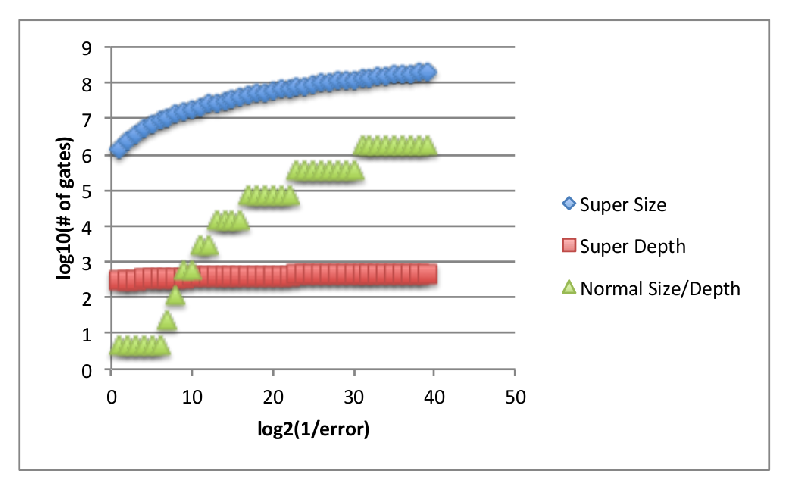
\includegraphics[width=3in]{circuit-size-depth.eps}
\caption{Compiled circuit size and depth}
\end{figure}
\end{center}

The tradeoff between Solovay-Kitaev and Super-Kitaev can most clearly
be seen in the use of space. Solovay-Kitaev uses no ancillae at run-time,
but requires a classical preprocessing step to generate basic
approximations (precompiled sequences from the universal set). Although
we did not generate sequences beyond $l_0 = 9$ for $SU(4)$, the curve
indicates it would soon require terabytes of storage, even if a more
efficient encoding were used (e.g. programming in C instead of Python).
Super-Kitaev, on the other hand, requires no preprocessing space, but
has a (currently intractable) requirement for ancilla qubits are run-time
which tracks the circuit size as $O(n^2 \log n)$.

\begin{center}
\begin{figure}[h!]
\label{fig:generation}
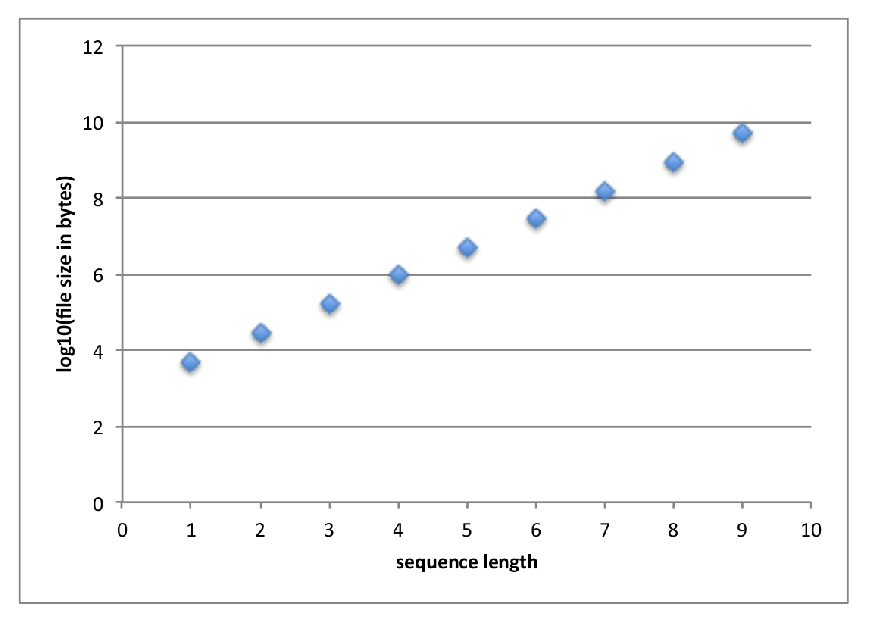
\includegraphics[width=3in]{normal-generation.eps}
\caption{Solovay-Kitaev preprocessing file sizes}
\end{figure}
\end{center}

\begin{center}
\begin{figure}[h!]
\label{fig:ancilla}
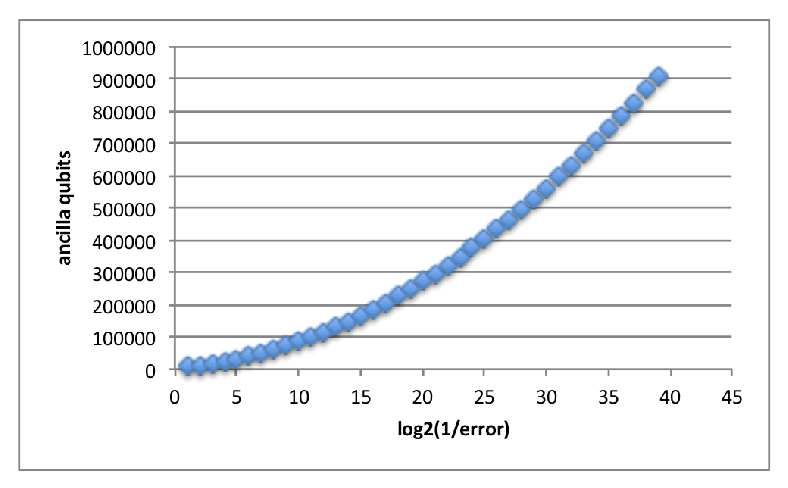
\includegraphics[width=3in]{super-ancilla.eps}
\caption{Super-Kitaev ancilla}
\end{figure}
\end{center}


\section{Conclusion and Future Directions}

In summary, we have seen the expected asymptotic bounds of both the
Solovay-Kitaev and Super-Kitaev quantum compiling algorithms reflected in
numerical resource comparisons. Solovay-Kitaev requires a large classical
preprocessing overhead but produces a more tractable number of compiled
gates and zero ancillae, albeit at larger circuit depth. This seems to be
a more reasonable choice for early experiments in running algorithms on an
80-qubit ion-trap quantum computer, where physical trapping constraints
make large numbers of qubits problematic but we are potentially willing to
wait a long time for the computation to complete. On the other hand, the
situation may change in the future when
quantum computers become more mature, scalable, and parallel;
when we become more ambitious in our
algorithm input sizes; and when the performance bottleneck becomes circuit depth.
In that case, Super-Kitaev may be preferrable.
Quantum computer engineers of the future will be able to use this work to
choose the most suitable quantum compiling technique currently available
as well as compare it to future compiling algorithms.

Moreover, the development of a compiler is intertwined with the
development of the underlying architecture. Just as classical programming
languages hint at what features would be desirable to move out of software
(and compile-time)
and into hardware (and run-time), Super-Kitaev provides some suggestions
to future quantum architectures. Hardware which seeks to take advantage of
this low-depth compiling would need to have a
"phase factory" for enacting the $\Lambda(e^{i\phi})$ gate, which would
included an efficient parallelized phase estimation routine. These are
novel resources which are currently not being considered in related literature.

Furthermore, quantum compiling may provide some hints to how we can program
their analog cousins. Although analog computers have fallen out of
favor as a primary computing model due to noise problems, they are making a
resurgence as a complementary ``coprocessor'' to digital computers, much like
the imagined future role of quantum computers. Like quantum computers,
analog computing uses existing physical properties to perform useful
computation, such as solving differential equations using electric current
and potential. Multiple AC signals and a single DC signal can coexist
in superposition on a wire,
and complex impedance from resistors, capacitors, and inductors
can differentiate between components of different frequencies.

\begin{displaymath}
V = I(R + \frac{1}{j\omega_1 C} + j\omega_2 L + \ldots)
\end{displaymath}

While it is unlikely that such a model would be more powerful in general
from a computational complexity point of view, we may be able to use them
as a practical aid in solving specific engineering problems, such as
encoding the periods of cyclic integer groups in corresponding periods of
sinusoidal signals. Such an analog computing model might be able to be
programmed via recursive successive approximation like Solovay-Kitaev or
using the techniques of Super-Kitaev.

\section{Acknowledgements}

The author would like to gratefully acknowledge the help of
his advisors Dave Bacon and Mark Oskin,
as well as Aram Harrow for the introduction to
Super-Kitaev and related expertise.

\bibliography{report}
\bibliographystyle{tocplain}

\end{document}
